\documentclass[xcolor=x11names,compress,t]{beamer}

%% Beamer Packages %%%%%%%%%%%%%%%%%%%%%%%%%%%%%%%%
\usepackage{graphicx}

%% Beamer Layout %%%%%%%%%%%%%%%%%%%%%%%%%%%%%%%%%%
%\useoutertheme[subsection=false,shadow]{miniframes}
\useinnertheme{default}
\usefonttheme{serif}
\usepackage{cancel}
\usepackage{palatino}

\setbeamerfont{title like}{shape=\scshape}
%\setbeamerfont{frametitle}{shape=\scshape}

\definecolor{ncsablue}{RGB}{12,81,156}

\setbeamercolor*{lower separation line head}{bg=gray}
\setbeamercolor*{normal text}{fg=black,bg=white}
\setbeamercolor*{alerted text}{fg=red}
\setbeamercolor*{example text}{fg=black}
\setbeamercolor*{structure}{fg=black}
\setbeamercolor*{title}{fg=black}
\setbeamercolor*{titlelike}{fg=ncsablue}
 
\setbeamercolor*{palette tertiary}{fg=black,bg=black!10}
\setbeamercolor*{palette quaternary}{fg=black,bg=black!10}

\beamertemplatenavigationsymbolsempty
\setbeamertemplate{footline}[page number]

\renewcommand{\(}{\begin{columns}}
\renewcommand{\)}{\end{columns}}
\newcommand{\<}[1]{\begin{column}{#1}}
\renewcommand{\>}{\end{column}}
%%%%%%%%%%%%%%%%%%%%%%%%%%%%%%%%%%%%%%%%%%%%%%%%%%

\begin{document}

\abovedisplayskip=6pt

%%%%%%%%%%%%%%%%%%%%%%%%%%%%%%%%%%%%%%%%%%%%%%%%%%%%%%
%%%%%%%%%%%%%%%%%%%%%%%%%%%%%%%%%%%%%%%%%%%%%%%%%%%%%%
%
% FRONT MATTER AND INTRODUCTION
%

\begin{frame}
\title{Obstacle Avoidance for a Quadrotor}
%\subtitle{ }
\author{Nikoli Dryden \and Bryan Plummer}
\date{}
\titlepage
\end{frame}

%%%%%%%%%%%%%%%%%%%%%%%%%%%%%%%%%%%%%%%%%%%%%%%%%%%%%%

\begin{frame}
  \frametitle{Introduction}
  \begin{itemize}
  \item Obstacle avoidance for an ARDrone 2.0 quadrotor
  \item Use the approach in \emph{Obstacle avoidance for small UAVs using monocular vision} (Lee et al. 2011)
  \item Test with real data as opposed to simulations
  \end{itemize}
\end{frame}

\begin{frame}
  \frametitle{Proposed Solution}
  \begin{itemize}
  \item Extract SIFT and MOPS features from two images
  \item Match SIFT and MOPS features in images to locate points in 3D
  \item Use MOPS to get object outlines
  \item Use SIFT to get internal object structure
  \item Determine type of object
  \end{itemize}
\end{frame}

\begin{frame}
  \frametitle{MOPS}
  \begin{itemize}
  \item Multi-Scale Oriented Patches (\emph{Image Matching using Multi-Scale Oriented Patches} (Brown et al. 2004))
  \item Detect features with multi-scale Harris corner detector
  \item Compute $8 \times 8$ patches of bias/gain normalized intensity values
  \item Orient using a blurred local gradient
  \end{itemize}
  \begin{center}
    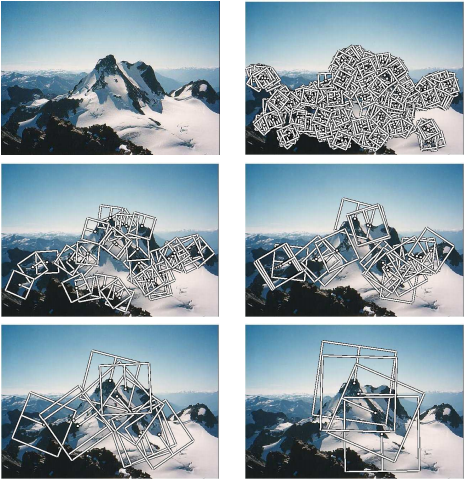
\includegraphics[resolution=150, scale=0.65]{images/mops-features.png}
  \end{center}
\end{frame}

\begin{frame}
  \frametitle{Some Results: SIFT}
  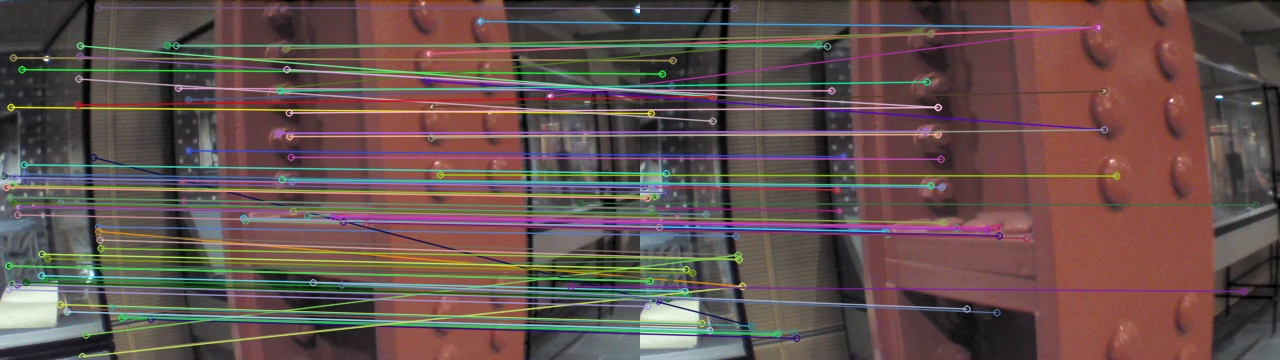
\includegraphics[resolution=150, scale=0.52]{images/sift-matches.jpg}
\end{frame}

\begin{frame}
  \frametitle{Some Results: MOPS}
  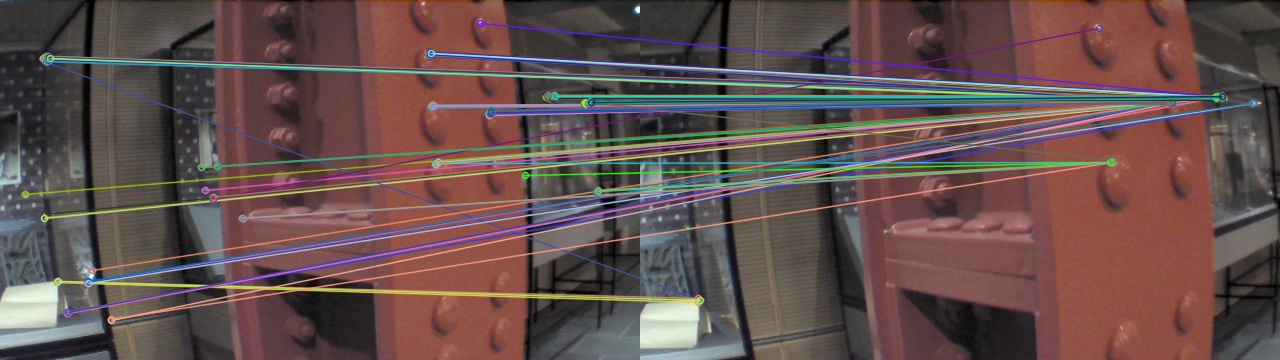
\includegraphics[resolution=150, scale=0.52]{images/mops-matches.jpg}
\end{frame}

\begin{frame}
  \frametitle{Some Results}
  \begin{itemize}
  \item MOPS is not robust on real data:
    \begin{itemize}
    \item Poor keypoints (multi-scale Harris)
    \item Poor matches
    \item Computationally intensive
    \end{itemize}
  \item SIFT is also relatively slow
  \item Do not have sufficient ``good'' matches to generate object outlines
  \item Lee et al. approach is not robust on real-world data
  \end{itemize}
\end{frame}

\begin{frame}
  \frametitle{A Better Idea}
  \begin{itemize}
  \item Use faster and more robust features than SIFT and MOPS
  \item PTAM
    \begin{itemize}
    \item An existing monocular SLAM framework using FAST (and other) features
    \item Robust enough to work with real-world indoor and outdoor data
    \item Significantly faster than our approach
    \end{itemize}
  \item Integrate with the quadrotor using ardrone\_autonomy and tum\_ardrone
  \end{itemize}
\end{frame}

\begin{frame}
  \frametitle{Further Results}
  TODO: Images/video from flight
\end{frame}

\begin{frame}
  \frametitle{Conclusions}
  \begin{itemize}
  \item MOPS is slow and not robust
  \item The Lee, et al. approach is not robust on the quadrotor
  \item PTAM works well
  \end{itemize}
\end{frame}

%%%%%%%%%%%%%%%%%%%%%%%%%%%%%%%%%%%%%%%%%%%%%%%%%%%%%%

\end{document}